\documentclass[dvips,xcolor=pst,14pt]{beamer}
%\documentclass[dvips,handout,xcolor=pst]{beamer}
%\documentclass[letterpaper]{article}
%\usepackage{beamerarticle}
\newcommand{\newblock}{}
\usepackage{pstricks}
%\usepackage{hyperref}
%\usepackage[authoryear]{natbib}
\usepackage{graphicx}
\usepackage{multimedia}
\usepackage{pgfpages}
\usepackage{arydshln}
\usepackage{commath}
\usepackage{vector}
%\usepackage{cancel}
\usepackage{ulem}
\usepackage{listings}
\usepackage{fancyvrb}
%\usepackage{times}

\graphicspath{{solvcon_eps/}}

\newcommand{\defeq}{\ensuremath{\buildrel {\text{def}}\over{=}}} 

%\usetheme{Berlin}
%\usetheme{Boadilla}
%\usetheme{Luebeck}
%\usetheme{Pittsburgh}
\usetheme{CambridgeUS}
%\usecolortheme{seagull}
%\setbeameroption{show notes}
%\setbeameroption{show only notes}
%\pgfpagesuselayout{2 on 1}[letterpaper,border shrink=0.2in]
%\usefonttheme[stillsansseriftext]{serif}
\usefonttheme[onlymath]{serif}

\title[SOLVCON: HPC PDE Solvers]{Implement High-Performance PDE Solvers for
First-Principle Simulations by Using Python}
%
\author[\href{http://solvcon.net/yyc/}{Chen}]%
{\href{http://solvcon.net/yyc/}{Yung-Yu Chen} \\ \url{yyc@solvcon.net}}
%
\institute[\href{http://solvcon.net/}{SOLVCON}]%
{Developer \\ \href{http://solvcon.net/}{SOLVCON Project}}
%
\date[2012/9/19]{PyCon Japan 2012 \\ September 16}

\begin{document}

\begin{frame}
\titlepage
\end{frame}

\section*{
%%%
Outline
%%%
}

\begin{frame}{
%
Whom I Am and What's This About
%
}
\begin{itemize}
  \item I am a numerical analyst, a computational scientist, a Python programmer.
  \begin{itemize}
    \item I am going to talk about \alert{SOLVCON}.
  \end{itemize}
  \item SOLVCON: Constructor of conservation-law \\ solvers.
  \begin{itemize}
    \item Perform first-principle simulations that are governed by conservation
    laws.
    \item Address \alert{high-performance computing (HPC)} by mesh-based,
    array-oriented programming.
    \item Implemented in Python and accelerated by C and other low-level tools.
  \end{itemize}
\end{itemize}
\end{frame}

\begin{frame}{
%
What Do I Want to Do with Python
%
}
\begin{itemize}
  \item Writing (fully-fledged) first-principle solvers is time-consuming.
  \begin{itemize}
    \item And it doesn't always work.  Sigh.
  \end{itemize}
  \item Can I use Python (in SOLVCON) to ease the pain?
  \begin{itemize}
    \item I am not along: Check \href{http://www.fenicsproject.org/}{FEniCS}
    and \href{http://www.ctcms.nist.gov/fipy/}{FiPy}.
  \end{itemize}
  \item \alert{HPC} is a primary concern of SOLVCON.
  \begin{itemize}
    \item Hundreds, thousands, and hopefully hundreds of thousands of nodes.
  \end{itemize}
\end{itemize}
\end{frame}

\begin{frame}{
%
Outline
%
}
\tableofcontents
\end{frame}

\section{
%%%
Background
%%%
}

\subsection{
%%
First-Principle Simulations and Conservation Laws
%%
}

\begin{frame}{
%
Conservation Laws Govern The World
%
}
\begin{center}
  Fluid mechanics, solid mechanics, electromagnetism, etc.
  \begin{minipage}{0.32\textwidth} \centering
  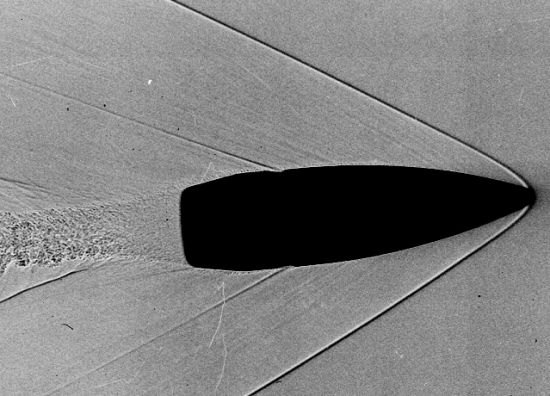
\includegraphics[width=\textwidth]{supersonic_bullet.eps} \\
  \small Supersonic flow.
  \end{minipage}
  \hskip 1em
  \begin{minipage}{0.32\textwidth} \centering
  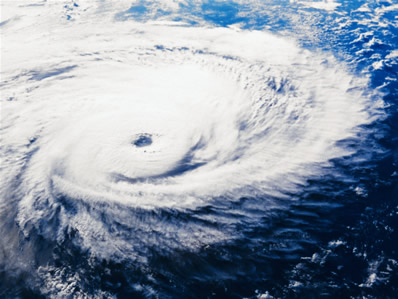
\includegraphics[width=\textwidth]{climate.eps} \\
  \small Atmospheric flow.
  \end{minipage}
  \hskip 1em
  \begin{minipage}{0.25\textwidth} \centering
  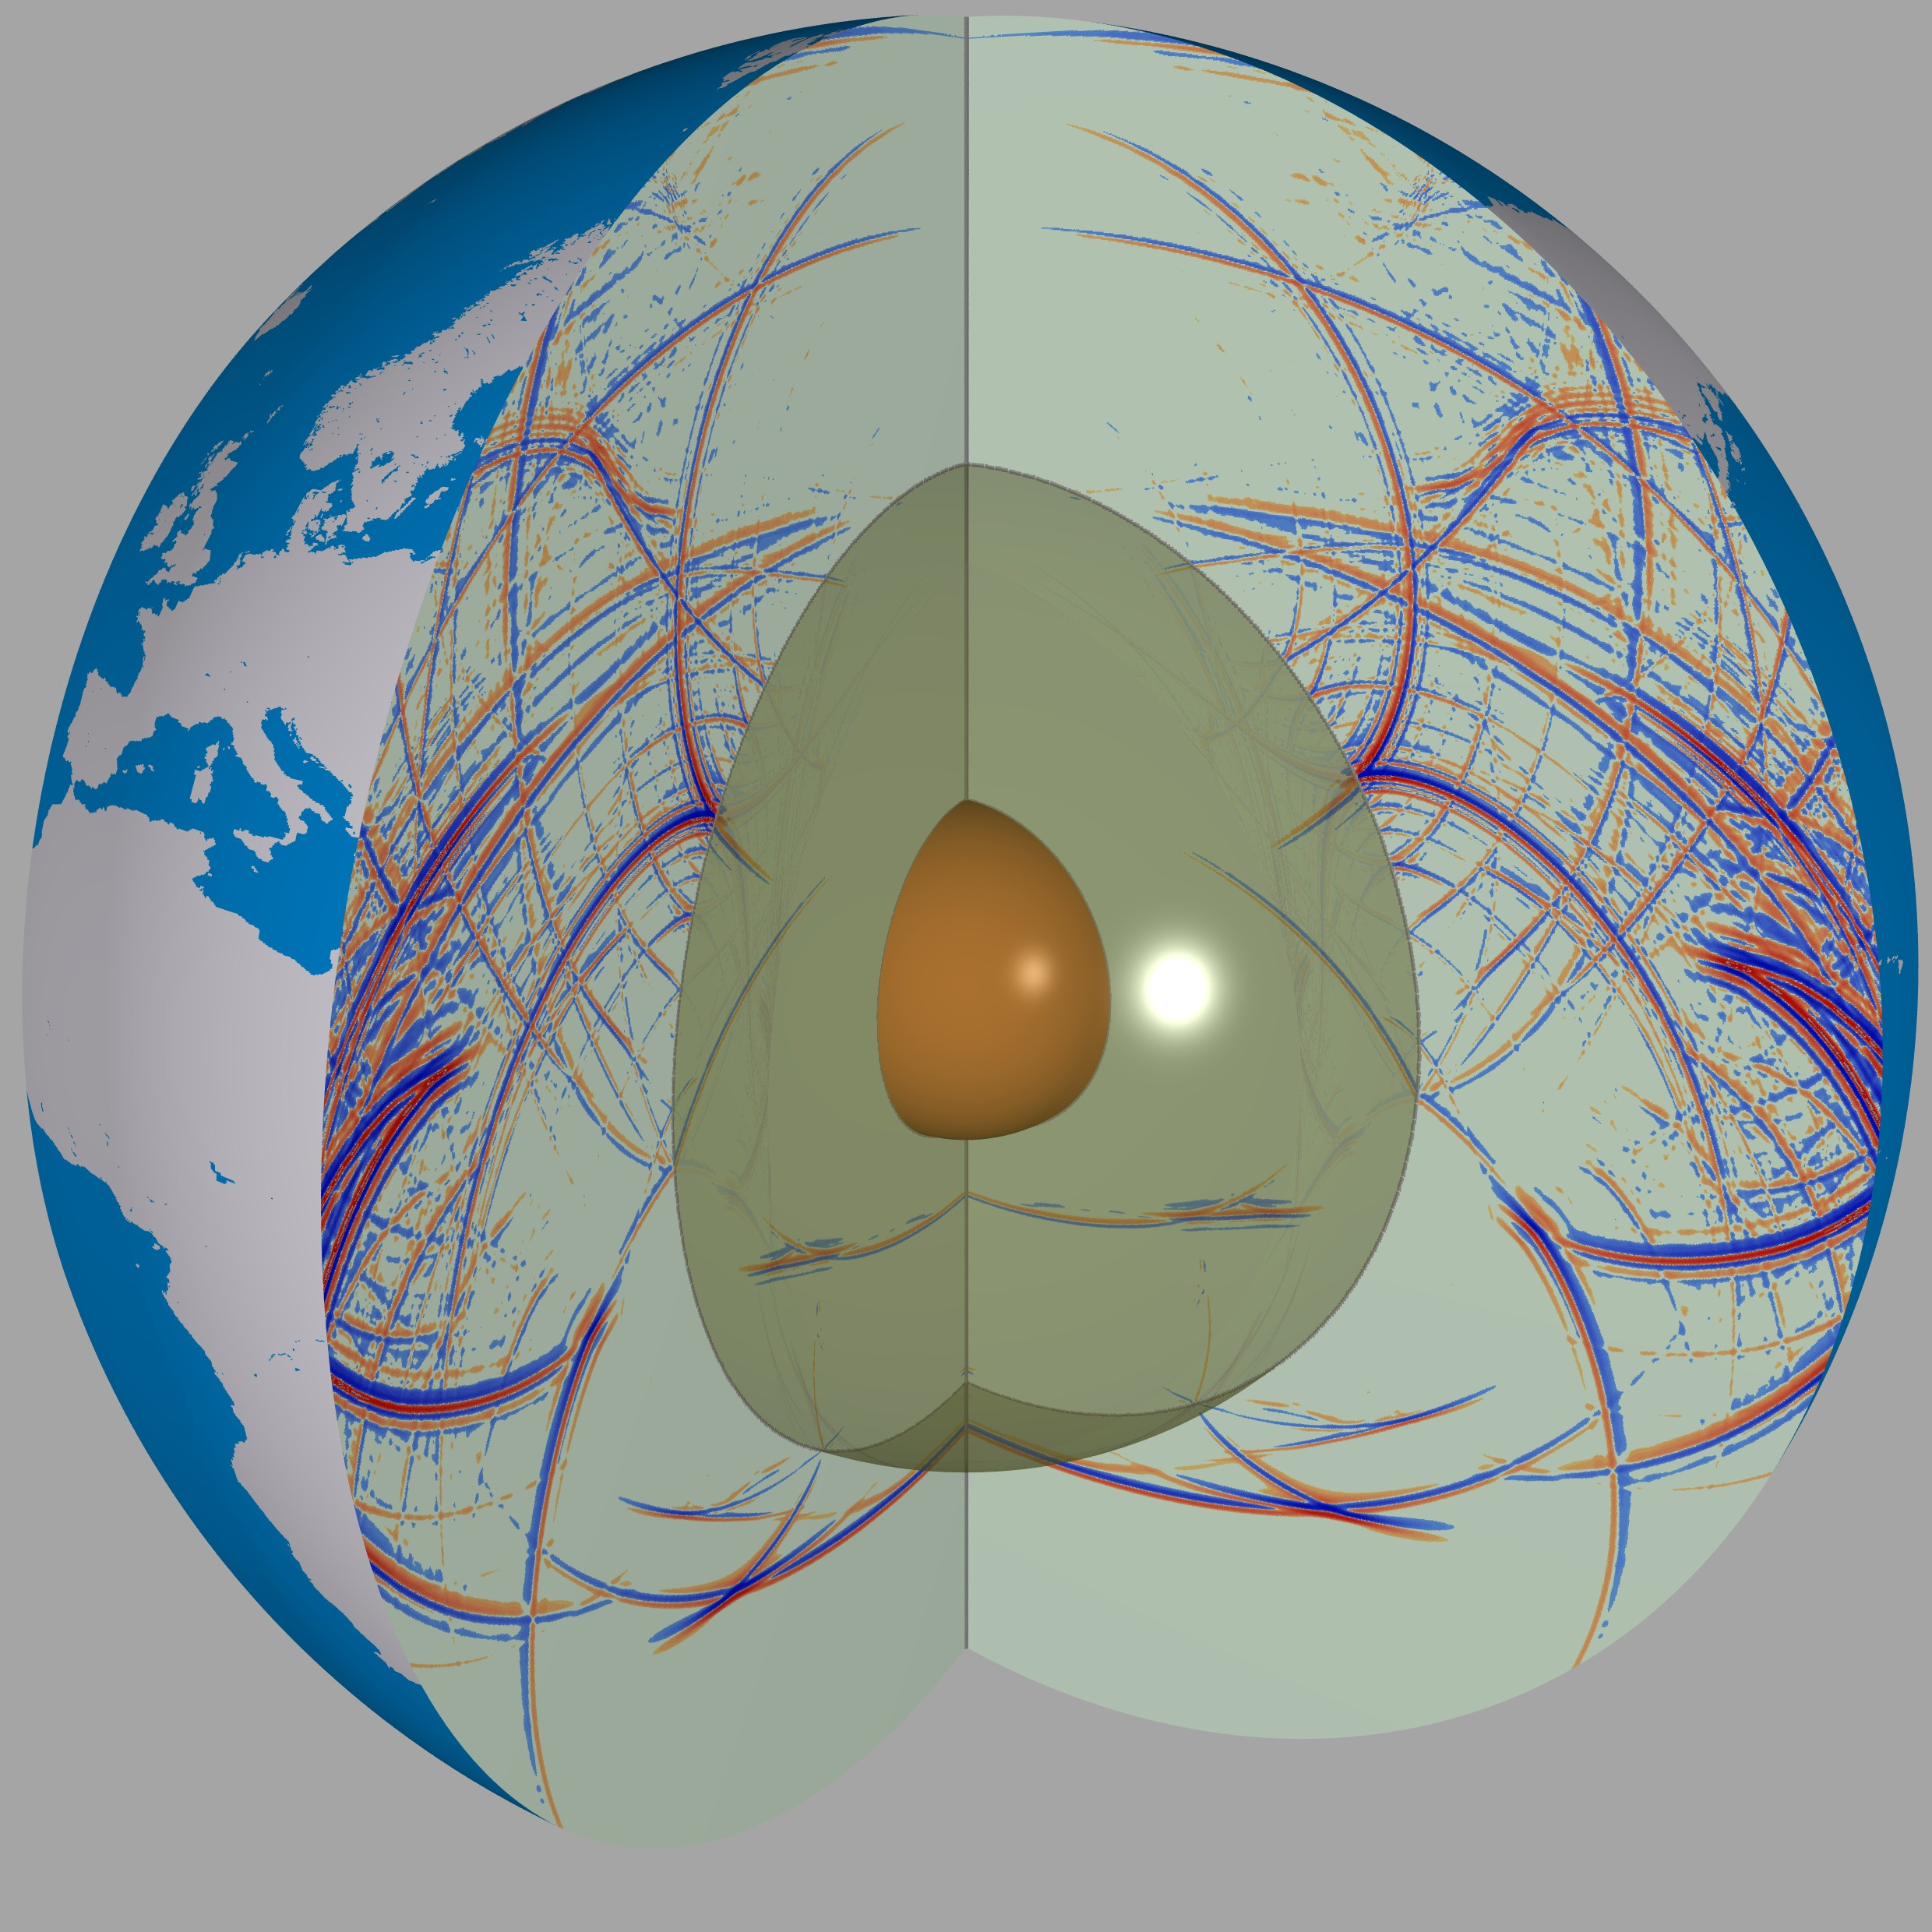
\includegraphics[width=\textwidth]{seismic_wave.eps} \\
  \small Seismic waves.
  \end{minipage}
\end{center}
\begin{center}
  \begin{minipage}{0.4\textwidth} \centering
  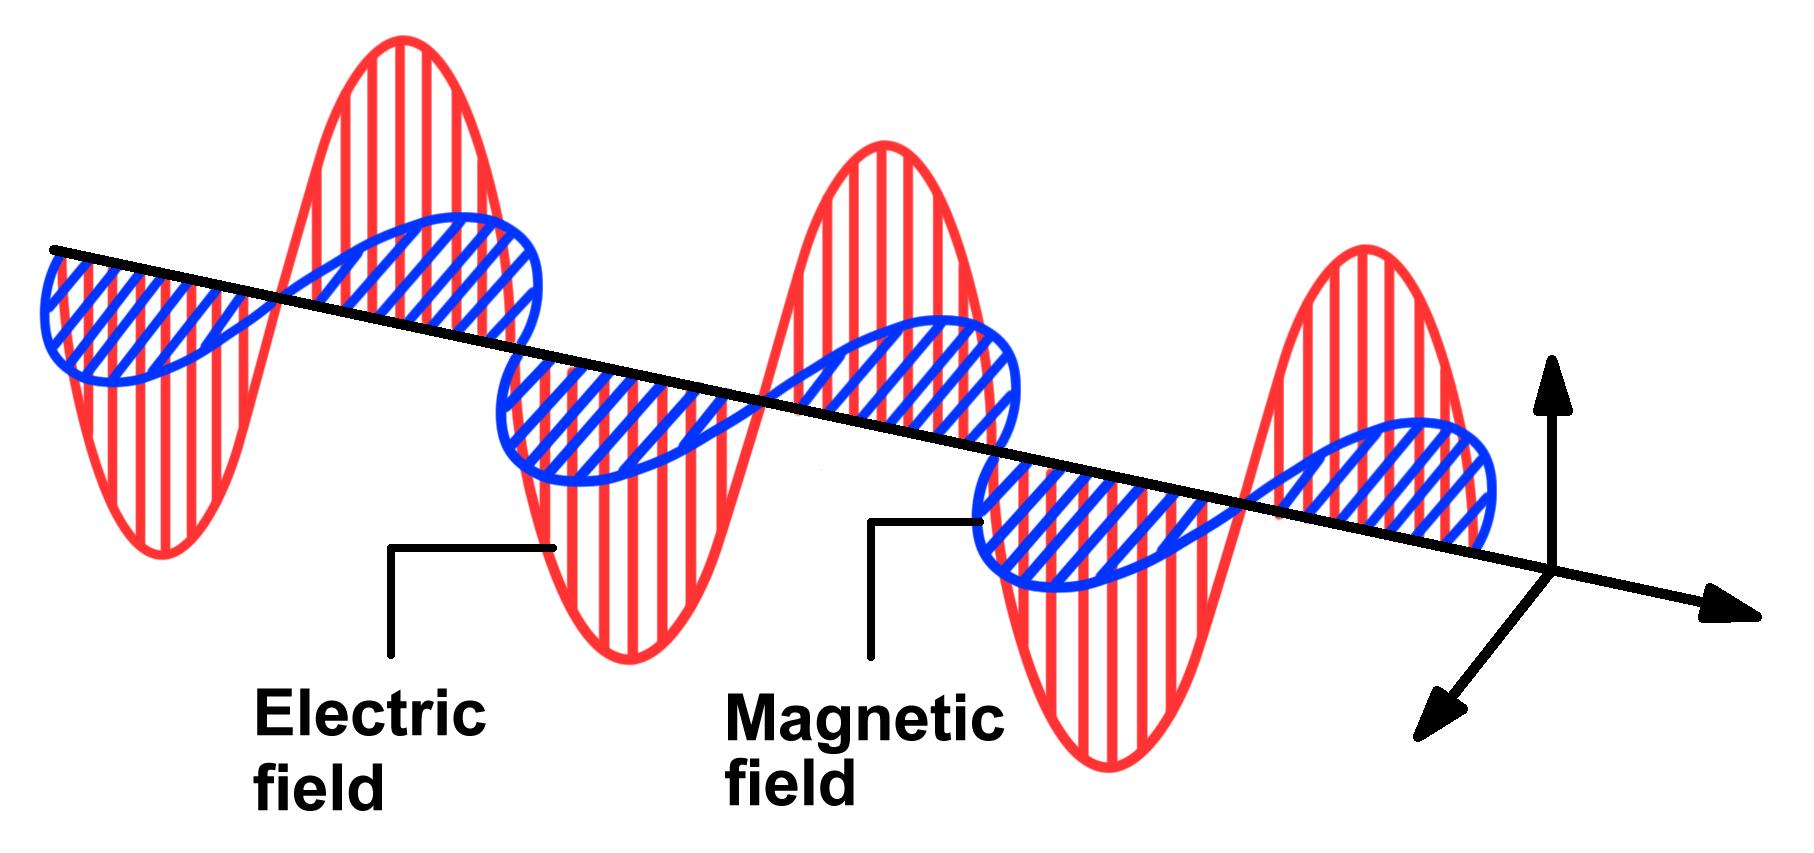
\includegraphics[width=\textwidth]{emwave.eps} \\
  \small Electromagnetic waves.
  \end{minipage}
\end{center}
\end{frame}

\begin{frame}{
%
Experiments?
%
}
\begin{center}
  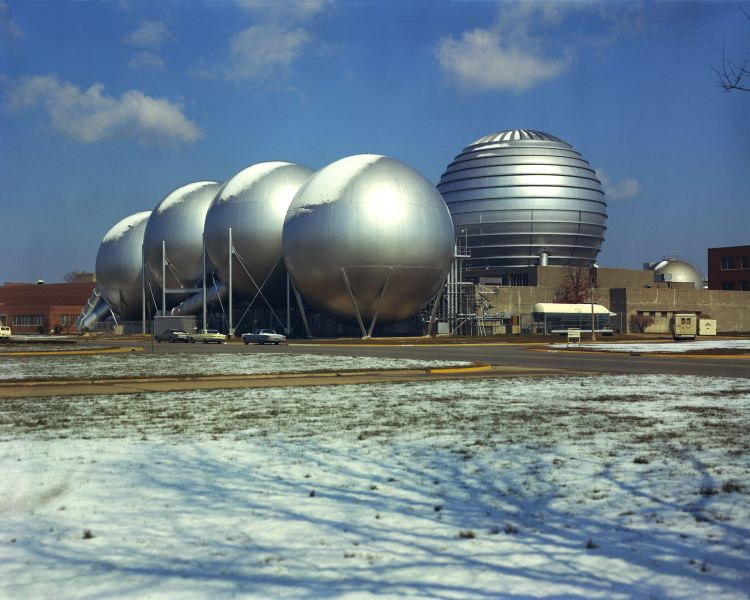
\includegraphics[width=0.7\textwidth]{Langley_hypersonic_wind_tunnels.eps} \\
  \href{http://en.wikipedia.org/wiki/Hypersonic_wind_tunnel}{Hypersonic Wind
  Tunnel (Mach 5+)}
\end{center}
\end{frame}

\begin{frame}{
%
Experiments, Seriously?
%
}
\begin{center}
  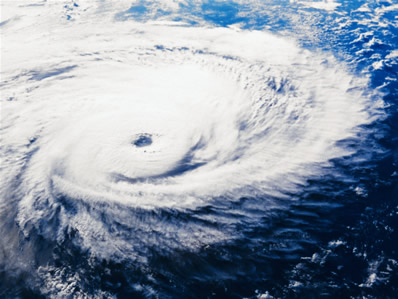
\includegraphics[width=0.8\textwidth]{climate.eps}
\end{center}
\end{frame}

\begin{frame}{
%
First-Order Hyperbolic PDEs
%
}
\begin{itemize}
  \item The fore-mentioned problems share a common trait: Demanding
  time-accurate solutions of conservation laws.
  \begin{itemize}
    \item These conservation laws can be cast into a system of full-coupled,
    first-order, linear or nonlinear, hyperbolic partial differential
    equations (PDEs).
    \item The nonlinearity adds a lot of $\mathcal{FUN}$.
  \end{itemize}
  \item So this is what I want to solve:
  {\footnotesize \begin{align}
   &\frac{\partial u_m}{\partial t}
      + \sum_{\mu=1}^3\frac{\partial f^{(\mu)}_m(\bvec{u})}{\partial x_{\mu}}
      = s_m(\bvec{u})
    \Rightarrow \boxed{\begin{gathered}
      \oint_{S(V)}\bvec{h}_m(\bvec{u})\cdot d\bvec{a}
      = \int_{V}s_m(\bvec{u})dv
    \end{gathered}} \label{e:conserv} \\
   &m = 1, \ldots, M. \notag
  \end{align}}
\end{itemize}
\end{frame}

\subsection{
%%
Why Develop SOLVCON?
%%
}

\begin{frame}{
%
Now a Programming Problem
%
}
Coding for first-principle simulators is difficult.  Why?
\begin{enumerate}
  \item Recall the math:
  {\footnotesize \begin{align}
   \frac{\partial u_m}{\partial t}
      + \sum_{\mu=1}^3\frac{\partial f^{(\mu)}_m(\bvec{u})}{\partial x_{\mu}}
      = s_m(\bvec{u}) \tag{\ref{e:conserv}}
  \end{align}}
  \item Various approaches to meshing and the associated data structures.
  \item Data management and result analysis.
  \item Parallel programming for HPC.
\end{enumerate}
\end{frame}

\begin{frame}{
%
Why Write Code for Simulation?
%
}
Come on, there are many commercial codes.  Is it really needed to develop yet
another research code?
\begin{itemize}
  \item Yes, because without the access to the source code, a computational
  scientist can never fully trust the code she uses.
  \item Commercial codes always implement the algorithms that can serve a
  larger crowd.  We have to code the cutting-edge things by ourselves.
\end{itemize}
\end{frame}

\begin{frame}{
%
Open-Source Research Codes?
%
}
\begin{itemize}
  \item Plenty of research codes are open-source, although the use of the
  source code can be limited by the license.
  \begin{itemize}
    \item As the name suggests, many research codes lack the modern structure
    that allows reuse.
    \item 10 incompatible versions of a code in a research group?  Nobody likes
    it, but it's quite often.
  \end{itemize}
  \item Good codes like FEniCS and FiPy didn't focus on time-accurate solution
  of conservation laws with HPC.
  \begin{itemize}
    \item FEniCS is based on finite-element method (FEM).
    \item FiPy is based on projection method.
  \end{itemize}
\end{itemize}
\end{frame}

\begin{frame}{
%
And I Learned the CESE Method
%
}
\begin{itemize}
  \item The space-time Conservation Element and Solution Element
  (\href{http://www.grc.nasa.gov/WWW/microbus/}{CESE}) method, developed by
  Chang at NASA Glenn.
  \begin{itemize}
    \item Directly solves generic hyperbolic PDEs (Eq.~\eqref{e:conserv}).
    \item Explicit time-marching for time-accurate solutions.
  \end{itemize}
  \item Enable pluggable multi-physics in SOLVCON.
  \begin{itemize}
    \item Compressible flows: $\bvec{u} = (\rho, \rho v_1, \rho v_2, \rho v_3,
    \rho e)^t$.
    \item Stress waves in solids: $\bvec{u} = (v_1, v_2, v_3, \sigma_{11},
    \sigma_{22}, \sigma_{33}, \sigma_{23}, \sigma_{13}, \sigma_{12})^t$.
    \item Electromagnetic waves: $\bvec{u} = (E_1, E_2, E_3, B_1, B_2, B_3)^t$.
    \item Acoustics, shallow-water, viscoelasticity, etc.
  \end{itemize}
\end{itemize}

\begin{flushright}\footnotesize
\href{http://dx.doi.org/10.1006/jcph.1995.1137}{Chang (1995) Journal of
Computational Physics 119(2):295--324} \\
\href{http://solvcon.net/yyc/publications.html}{Chen (2011), Ph.D. Dissertation}
\end{flushright}

\end{frame}

\begin{frame}{
%
Scope of SOLVCON
%
}
\begin{itemize}
  \item A Python-based software framework for constructing time-accurate
  solvers of conservation laws for any physical processes.
  \item SOLVCON currently contains referential solvers that use the CESE method.
  \begin{itemize}
    \item Unstructured meshes of mixed elements are used in two- or
    three-dimensional space.
    \item Message-passing is built into the framework for parallel computing.
  \end{itemize}
  \item A PDE-solving toolkit supporting parallel computing that can be
  embedded into your application for delivering analyzed results.
\end{itemize}
\end{frame}

\subsection{
%%
Basics of SOLVCON
%%
}

\begin{frame}{
%
Introduce SOLVCON
%
}
\begin{itemize}
  \item Features:
  \begin{itemize}
    \item Pluggable multi-physics.
    \item Unstructured meshes for modeling complex geometry.
    \item Hybrid parallel computing.
    \item Ready-to-use I/O formats.
    \item Parallel I/O and in situ visualization.
    \item Automated work flow.
  \end{itemize}
  \item Architecture:
  \begin{itemize}
    \item Mesh-based programming for array-oriented computing.
    \item Two-loop structure.
    \item Inversion of control based on the mesh and two-loop.
  \end{itemize}
\end{itemize}
\end{frame}

\begin{frame}{
%
Application: Stress Wave in Solids
%
}
\begin{itemize}
  \item Beryl: Anisotropic crystal of hexagonal symmetry.
\end{itemize}
\begin{center}
  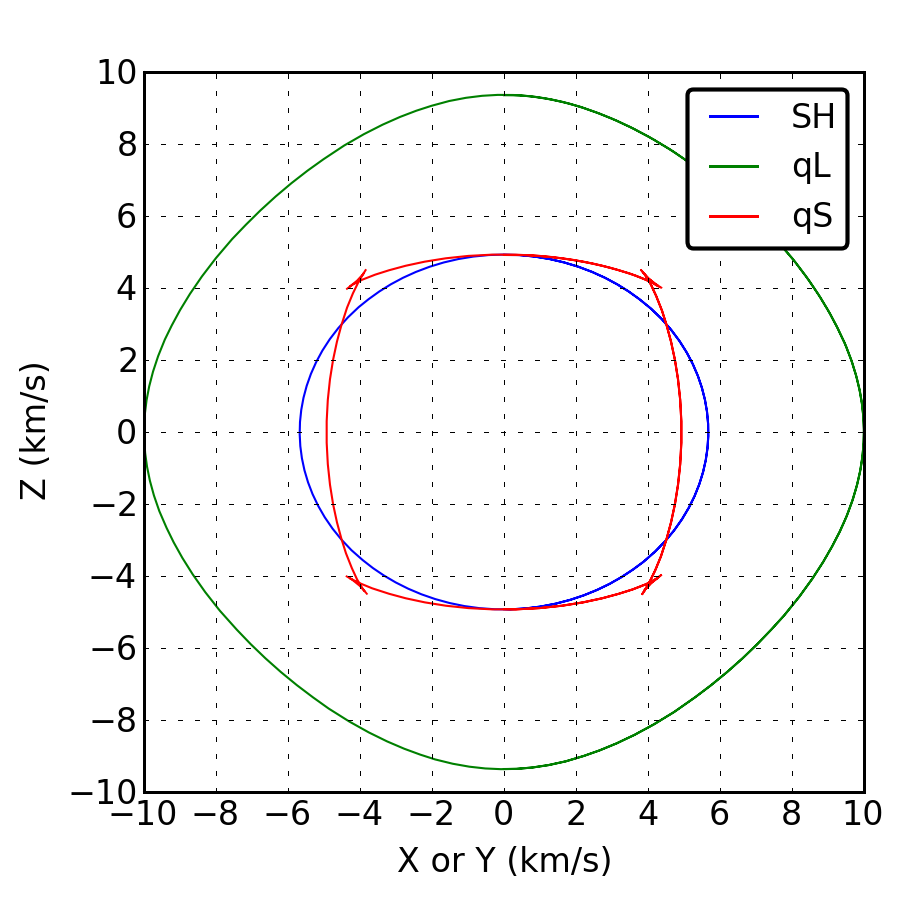
\includegraphics[width=0.4\textwidth]{Beryl.eps}
  \hskip 0.5em
  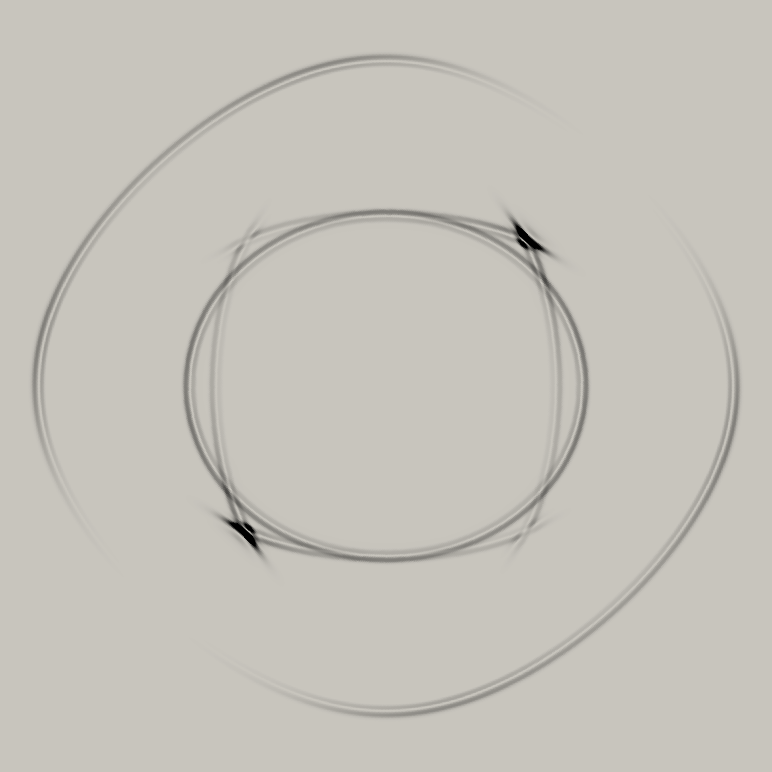
\includegraphics[width=0.4\textwidth]{Beryl_sim_white.eps}
  \\
  \parbox[t]{0.4\textwidth}{\footnotesize \centering Exact solution of group velocity}
  \hskip 1em
  \parbox[t]{0.4\textwidth}{\footnotesize \centering Simulated result}
\end{center}

\parbox{\textwidth}{\raggedleft \footnotesize
\href{http://dx.doi.org/10.1115/1.4002170}{Yang et al. (2011) J.  Vib. Acoust.
133(2): 021001}}
\end{frame}

\begin{frame}{
%
Application: Supersonic Flows
%
}
\begin{columns}[c]
\begin{column}{.6\textwidth}
\begin{center}
  \begin{minipage}[c]{\textwidth} \centering
    \parbox{0.3\textwidth}{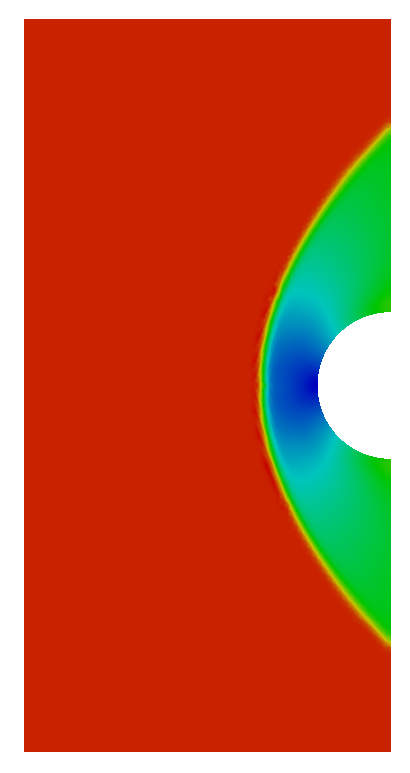
\includegraphics[width=0.3\textwidth]{foc_m3.eps}}
    \hfill
    \parbox{0.65\textwidth}{%
    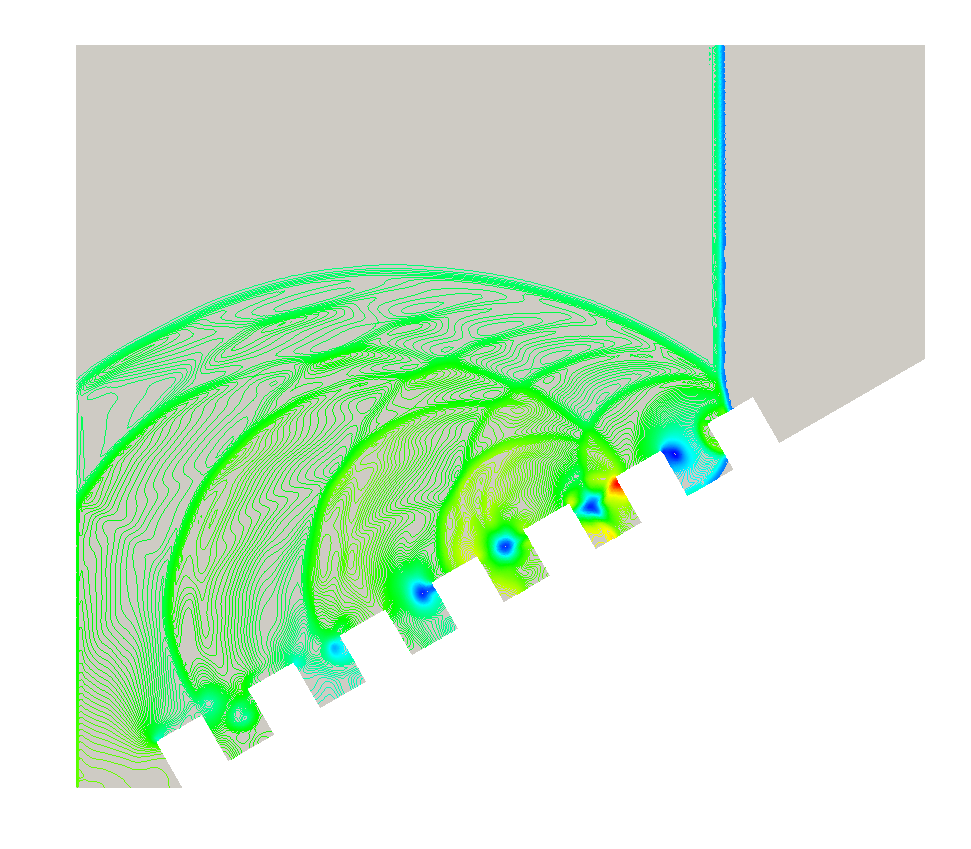
\includegraphics[width=0.65\textwidth]{dust_layer.eps}}
  \end{minipage} \\
  \begin{minipage}[c]{\textwidth} \centering
    \parbox{\textwidth}{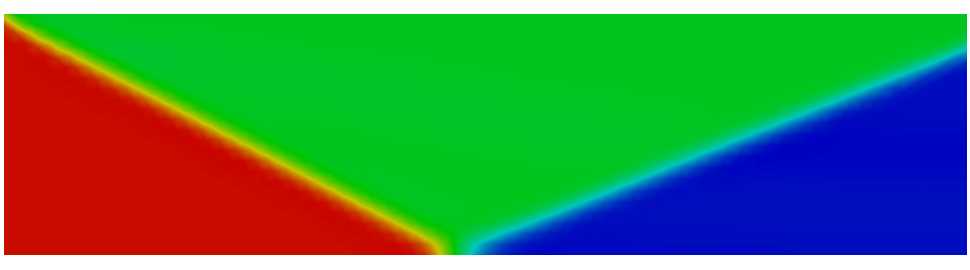
\includegraphics[width=\textwidth]{refl_m3.eps}}
  \end{minipage}
\end{center}\end{column}
\begin{column}{.4\textwidth}
\begin{itemize} \scriptsize
  \item 2D cases:
  \begin{itemize} \scriptsize
    \item Flow over a cylinder.
    \item Oblique shock by a ramp.
    \item Moving shock climbing a ramp.
    \item Moving shock diffraction by a step.
    \item Moving shock past dust layer.
    \item Reflection of oblique shock.
    \item Implosion.
  \end{itemize}
  \item 3D cases:
  \begin{itemize} \scriptsize
    \item Sod's shock tube.
    \item Flow over sphere.
    \item Jet in cross flow.
  \end{itemize}
\end{itemize}
\end{column}
\end{columns}
\end{frame}

\begin{frame}{
%
Jet in Supersonic Cross Flow
%
}
66 million elements are used in the simulation.
\begin{center}
  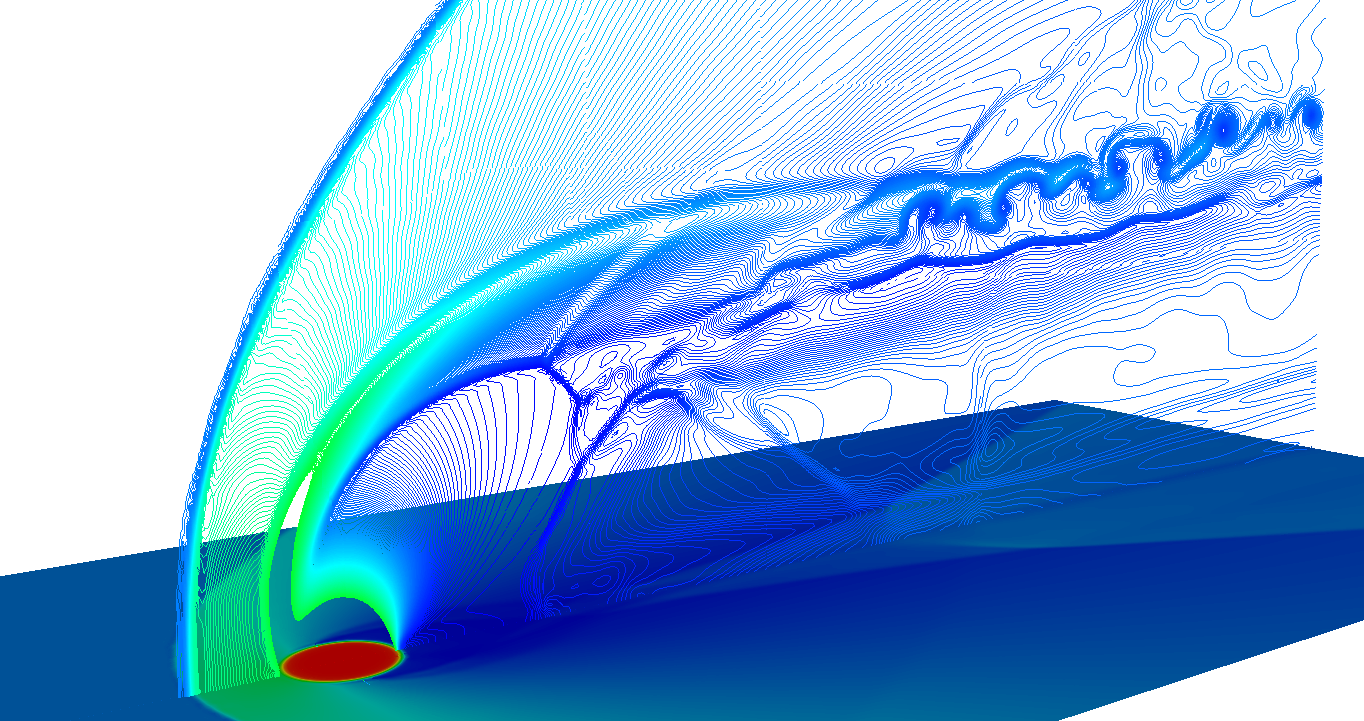
\includegraphics[width=0.9\textwidth]{pjcf_28_density.eps} \\
  \scriptsize Density
\end{center}
\end{frame}

\begin{frame}{
%
Runtime Benchmark
%
}
\begin{itemize}
  \item Benchmark with hybrid parallel computing.
  \begin{itemize}
    \item MPI across nodes; pthread within a node.
    \item Run on Glenn@OSC: 4 cores/node with 10Gbps IB.
  \end{itemize}
  \item Performance in million elements per second (Meps).
\end{itemize}
\begin{center} \footnotesize
  \begin{tabular}{ll|cccc}
  \multicolumn{2}{l|}{Number of cells (M)}
                            & 1     & 11   & 34   & 66   \\
  \hline
  Perf. (Meps) &    1 core  & 0.035 & --   & --   & --   \\
               &    4 cores & 0.13  & --   & --   & --   \\
               &   16 cores & 0.45  & 0.47 & --   & --   \\
               &   32 cores & --    & 0.91 & --   & --   \\
               &   44 cores & --    & 1.26 & 1.33 & --   \\
               &   80 cores & --    & --   & 2.16 & --   \\
               &  136 cores & --    & --   & 3.61 & 3.82 \\
               &  264 cores & --    & --   & --   & 7.17 \\
               &  512 cores & --    & --   & --   & 12.7 \\
               & 1024 cores & --    & --   & --   & 20.0
  \end{tabular}
\end{center}
\end{frame}

\begin{frame}{
%
Scaling
%
}
\begin{columns}[c]
\begin{column}{.5\textwidth}
\begin{center}
  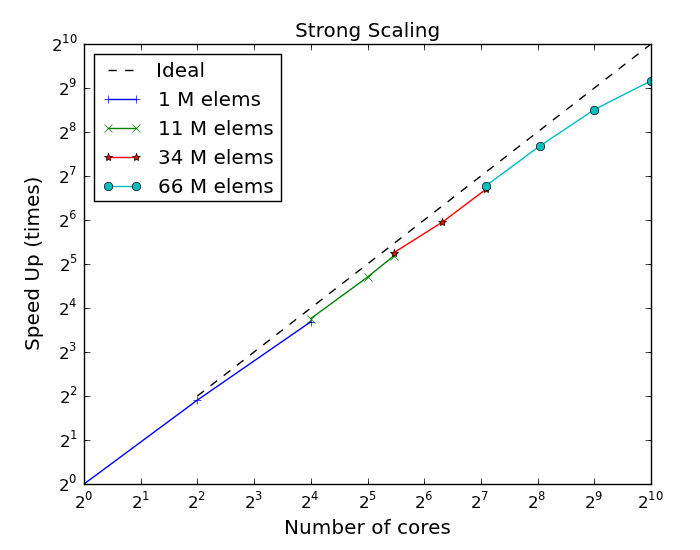
\includegraphics[width=\textwidth]{pjcf_speedup.eps} \\
  Fix Overall Mesh Size
\end{center}
\end{column}
\begin{column}{.5\textwidth}
\begin{center}
  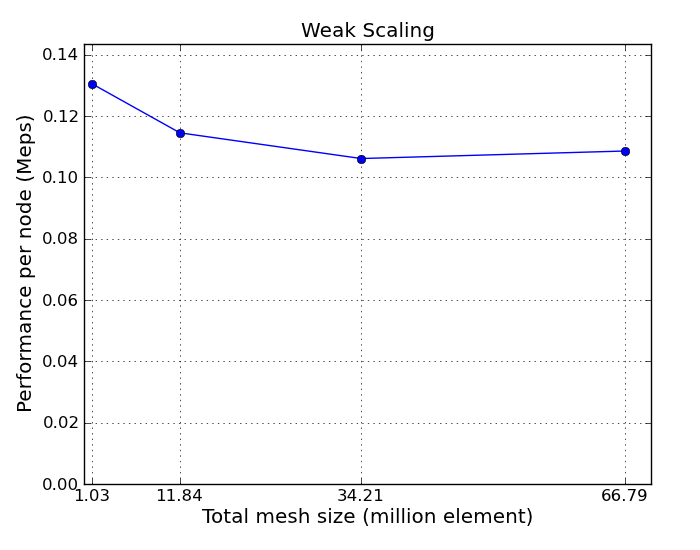
\includegraphics[width=\textwidth]{pjcf_weak.eps} \\
  Fix Per-Node Mesh Size
\end{center}
\end{column}
\end{columns}
\end{frame}

\section{
%%%
The Design of SOLVCON
%%%
}

\subsection{
%%
Mesh-Based Programming
%%
}

\begin{frame}{
%
Mesh-Based Programming
%
}
\begin{center}
  \begin{minipage}{0.19\textwidth} \centering
  \footnotesize Curvilinear \\
  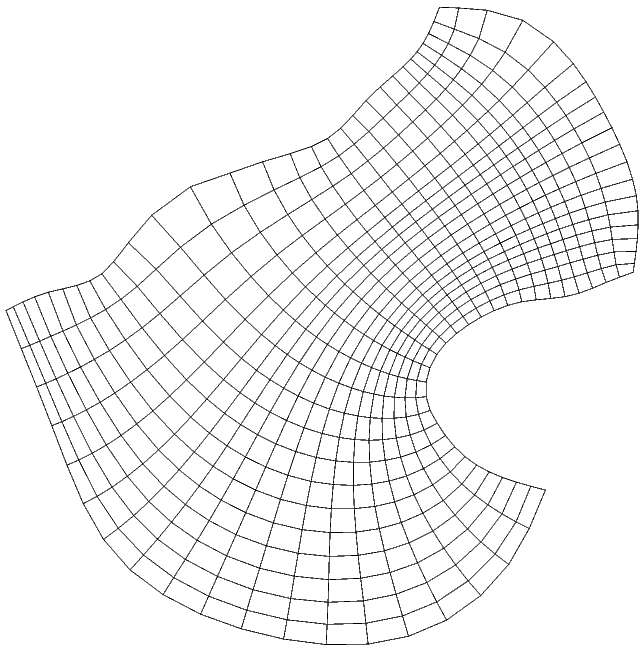
\includegraphics[width=0.8\textwidth]{structuredmesh.eps}
  \end{minipage}
  \hskip 0.5em
  \begin{minipage}{0.19\textwidth} \centering
  \footnotesize Cartesian \\
  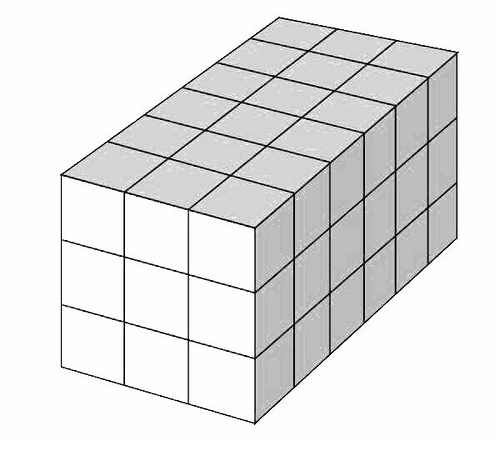
\includegraphics[width=\textwidth]{cartesianmesh.eps}
  \end{minipage}
  \hskip 2.5em
  \begin{minipage}{0.19\textwidth} \centering
  \footnotesize \alert{Unstructured} \\
  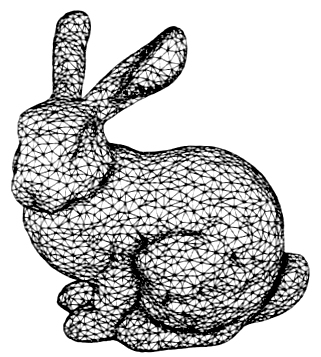
\includegraphics[width=0.8\textwidth]{unstructuredmesh.eps}
  \end{minipage}
\end{center}
\vskip -20pt
\begin{itemize}
  \item Two ways to discretize space:
  \begin{itemize}
    \item Structured mesh: The connectivity of elements is structured.
    Cartesian is a special case.
    \item Unstructured mesh: The connectivity of elements is \alert{irregular}.
  \end{itemize}
  \item SOLVCON uses \alert{unstructured mesh}:
  \begin{itemize}
    \item The data structure defines \textbf{connectivity} and
    \textbf{geometry}.
    \item Code is based on the data structure.
  \end{itemize}
\end{itemize}
\end{frame}

\begin{frame}{
%
Unstructured Meshes of Mixed Elements
%
}
\begin{itemize}
  \item Two-dimensional elements:
  \begin{center}
    \parbox{0.2\textwidth}{\centering
    \includegraphics[width=0.2\textwidth]{elm_tri.eps} \\ \footnotesize
    triangle}
    \parbox{0.2\textwidth}{\centering 
    \includegraphics[width=0.2\textwidth]{elm_quad.eps} \\ \footnotesize
    quadrilateral}
  \end{center}
  \item Three-dimensional elements:
  \begin{center}
    \parbox{0.2\textwidth}{\centering
    \includegraphics[width=0.2\textwidth]{elm_tet.eps} \\ \footnotesize
    tetrahedron}
    \parbox{0.2\textwidth}{\centering
    \includegraphics[width=0.2\textwidth]{elm_hex.eps} \\ \footnotesize
    hexahedron}
    \parbox{0.2\textwidth}{\centering
    \includegraphics[width=0.2\textwidth]{elm_psm.eps} \\ \footnotesize
    prism}
    \parbox{0.2\textwidth}{\centering
    \includegraphics[width=0.2\textwidth]{elm_pym.eps} \\ \footnotesize
    pyramid}
  \end{center}
\end{itemize}
\end{frame}

\begin{frame}{
%
Look-Up Tables for Meshes
%
}
\begin{columns}[c]
\begin{column}{.3\textwidth}
\begin{center}
  \includegraphics[width=\textwidth]{elm_tet.eps} \\ \footnotesize tetrahedron
\end{center}\end{column}
\begin{column}{.7\textwidth}
\begin{itemize}
  \item Consider cell-based solvers (value is stored at cell centers):
  \begin{itemize}
    \item 4 nodes for the cell: 0, 1, 2, 3.
    \item 4 faces for the cell: 012, 013, 123, 203.
  \end{itemize}
  \item Tables to connect all cells:
  \begin{itemize}
    \item Nodes in each cell (\texttt{clnds}).
    \item Faces in each cell (\texttt{clfcs}).
    \item Nodes in each face (\texttt{fcnds}).
    \item Cells connected by each face (\texttt{fccls}).
  \end{itemize}
\end{itemize}
\end{column}
\end{columns}
\end{frame}

\subsection{
%%
Two-Loop Structure
%%
}

\begin{frame}{
%
Two-Loop Structure of PDE Solvers
%
}
\begin{columns}[c]
\begin{column}{.5\textwidth}
\begin{itemize}
  \item The basic execution flow of SOLVCON:
  \begin{itemize}
    \item Temporal loop for temporal (or pseudo-temporal) integration.
    \item Spatial loops iterate over elements.
  \end{itemize}
  \item The structure is general to all PDE solvers.
\end{itemize}
\end{column}
\begin{column}{.5\textwidth}
  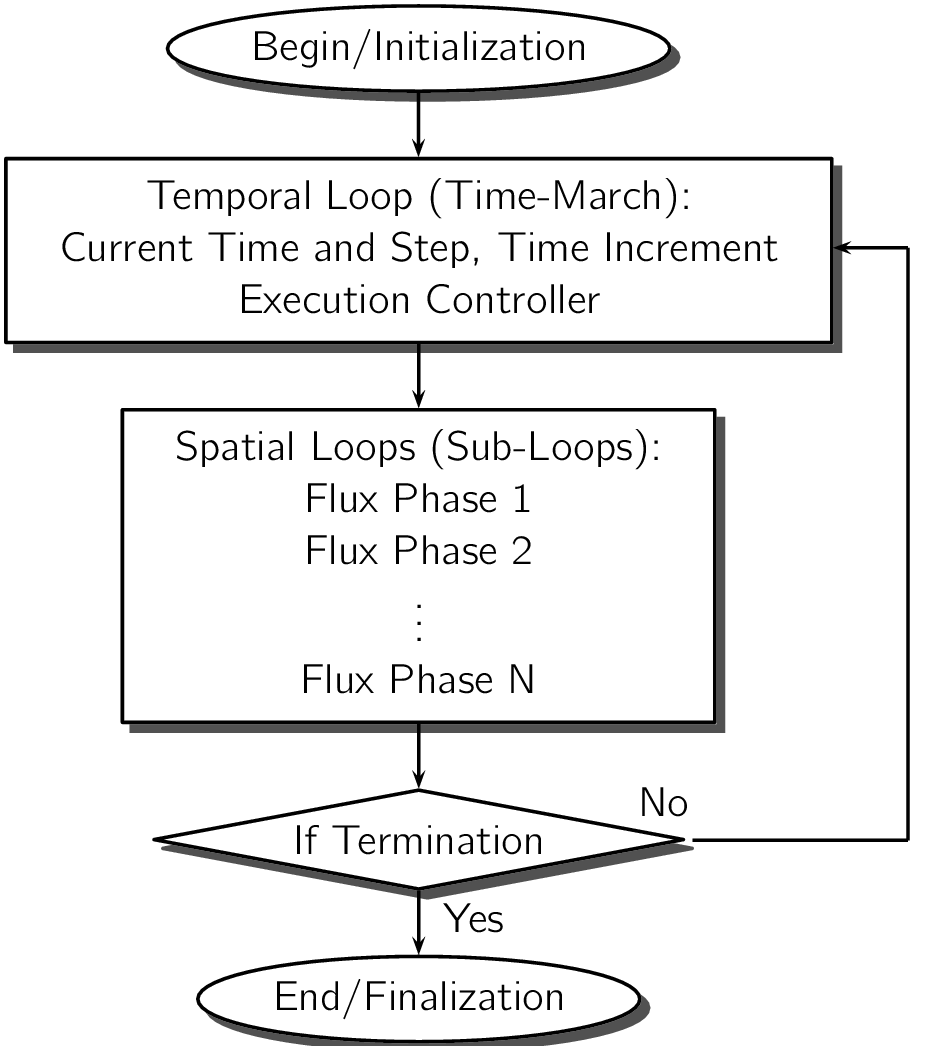
\includegraphics[width=.9\textwidth]{twoloop.eps}
\end{column}
\end{columns}
\end{frame}

\begin{frame}{
%
Solver Kernel for Spatial Loops
%
}
\begin{columns}[c]
\begin{column}{.75\textwidth}
\begin{itemize}
  \item A solver kernel is a Python class.
  \item The base class implements utility methods for \alert{spatial loops}.
  \item The concrete solver implements real algorithms.
  \item The algorithms directly work with the mesh look-up tables.
\end{itemize}
\end{column}
\begin{column}{.25\textwidth} \centering
  \includegraphics[width=\textwidth]{inheritance.eps}
\end{column}
\end{columns}
\end{frame}

\begin{frame}{
%
Inheritance for Multi-Physics
%
}
\begin{itemize}
  \item For a multi-physics algorithm, like the CESE method, a class hierarchy
  can be designed to host multiple physical processes.
\end{itemize}
\begin{columns}[c]
\begin{column}{.5\textwidth}
\begin{itemize}
  \item The physical processes are segregated.
\end{itemize}
\end{column}
\begin{column}{.5\textwidth} \centering
  \includegraphics[width=\textwidth]{mphysics.eps}
\end{column}
\end{columns}
\end{frame}

\begin{frame}{
%
Temporal Loop and Call-Back
%
}
\begin{itemize}
  \item A standalone class hierarchy (\texttt{Case}) is designed to host the
  \alert{temporal loop}.
\end{itemize}
\begin{center}
  \parbox{\textwidth}{\centering
  \includegraphics[width=\textwidth]{lazy.eps}}
\end{center}
\begin{itemize}
  \item \texttt{Hook} and \texttt{Anchor} are call-back objects for
  \texttt{Case} and \texttt{Solver}, respectively.
  \begin{itemize}
    \item Supplement of main algorithms.
    \item Lazy initialization.
    \item Facilitating parallel computing and in-situ analysis.
  \end{itemize}
\end{itemize}
\end{frame}

\begin{frame}{
%
Overall Design of SOLVCON
%
}
\begin{center}
  \parbox{\textwidth}{\centering
  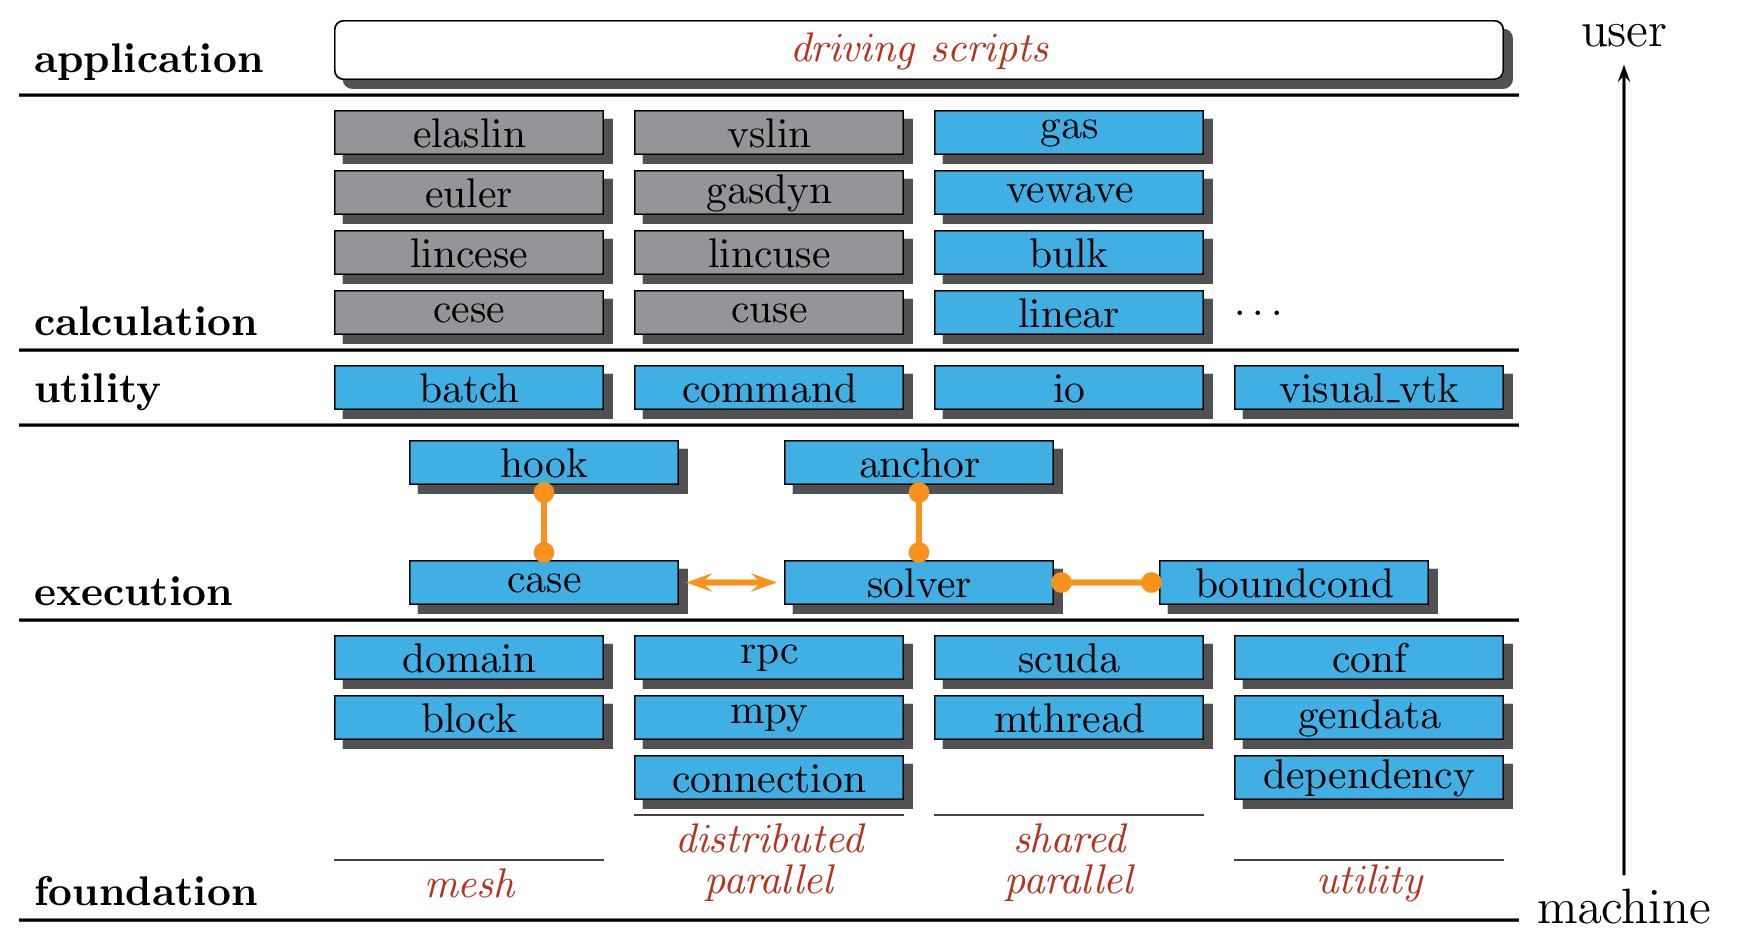
\includegraphics[width=\textwidth]{stack.eps}}
\end{center}
\end{frame}

\subsection{
%%
Parallel Computing
%%
}

\begin{frame}{
%
Two Types of Parallel Computing
%
}
\begin{minipage}[c]{\textwidth}\centering \footnotesize
\parbox{0.3\textwidth}{\centering
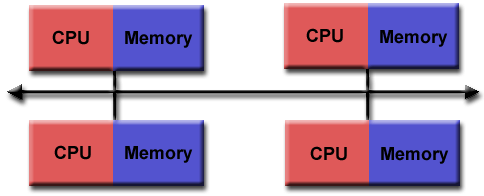
\includegraphics[width=0.3\textwidth]{mem_distributed.eps} \\ \footnotesize
distributed (cluster)}
+ 
\parbox{0.3\textwidth}{\centering 
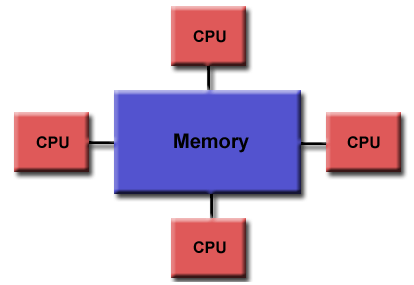
\includegraphics[width=0.3\textwidth]{mem_shared.eps} \\ \scriptsize shared
(multi-/many-core)}
= 
\parbox{0.3\textwidth}{\centering
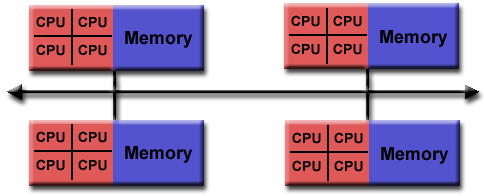
\includegraphics[width=0.3\textwidth]{mem_hybrid.eps} \\ \footnotesize hybrid}
\end{minipage}
\begin{itemize}
  \item Simultaneously use distributed-memory and shared-memory parallel
  computing (DMPC \& SMPC, respectively).
  \begin{itemize}
    \item Main difference: \alert{Addressing space}.
  \end{itemize}
  \item Inter-process communication is needed.
  \begin{itemize}
    \item \alert{MapReduce is unsuitable}.
    \item DMPC is much more complex than SMPC.
    \item \alert{DMPC determines the scalability}.
  \end{itemize}
\end{itemize}
\end{frame}

\begin{frame}{
%
Extending Solver Kernel for SMPC
%
}
\begin{columns}[c]
\begin{column}{.75\textwidth}
\begin{itemize}
  \item A \texttt{Solver} class can be extended to use shared-memory parallel
  computing.
  \item Only the spatial loops are modified.
  \item Can use pthread, OpenMP, CUDA, OpenCL, etc.
\end{itemize}
\end{column}
\begin{column}{.25\textwidth} \centering
  \includegraphics[width=\textwidth]{sharedmemory.eps}
\end{column}
\end{columns}
\end{frame}

\begin{frame}{
%
Domain Decomposition for DMPC
%
}
\begin{itemize}
  \item Before computation: Domain decomposition.
  \begin{itemize}
    \item Use connectivity data to build the graph of cells.
    \item Partition the graph by calling METIS or SCOTCH library.
    \item Use the partitioned graph to decompose mesh data.
  \end{itemize}
\end{itemize}
\begin{center} \scriptsize
  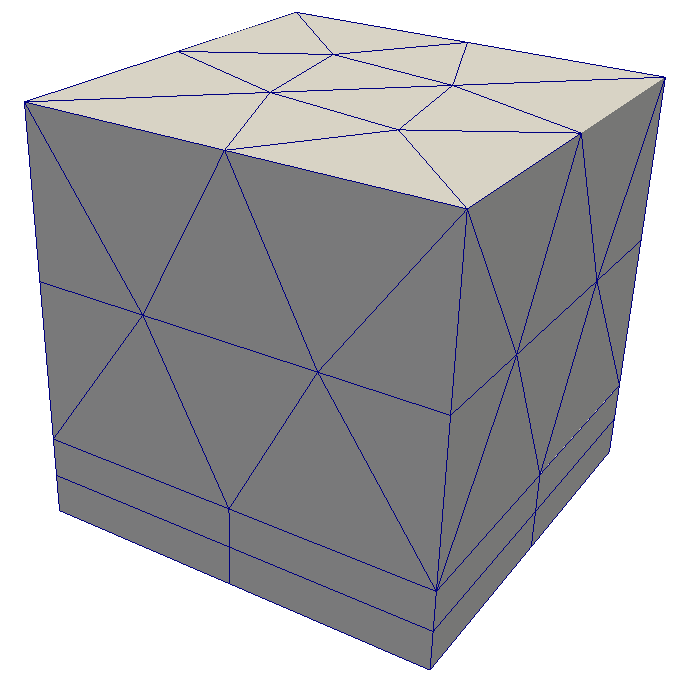
\includegraphics[width=0.2\textwidth]{mixed_mesh.eps}
  $\rightarrow$
  \includegraphics[width=0.25\textwidth]{meshgraph.eps}
  $\rightarrow$
  \includegraphics[width=0.25\textwidth]{meshgraph_partition.eps}
  $\rightarrow$
  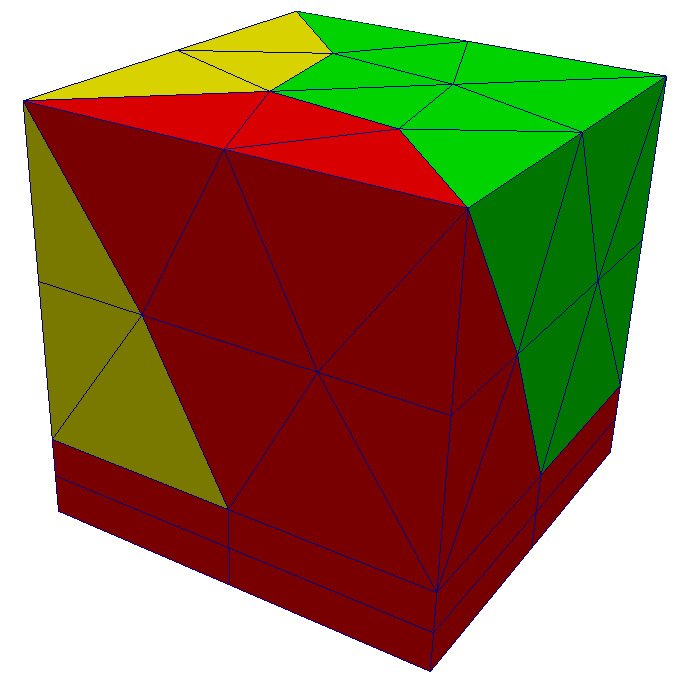
\includegraphics[width=0.2\textwidth]{mixed_mesh_decompose.eps}
\end{center}
\begin{itemize}
  \item During computation: Exchange data of the cells on the interface of
  different sub-domains.
  \begin{itemize}
    \item Use MPI to communicate among sub-domains.
  \end{itemize}
\end{itemize}
\end{frame}

\begin{frame}{
%
Solver Kernels Need Not Know DMPC
%
}
\begin{columns}[c]
\begin{column}{.3\textwidth}
\begin{itemize}
  \item DMPC is in SOLVCON framework.
  \item SMPC is in solver kernels.
\end{itemize}
\end{column}
\begin{column}{.7\textwidth} \centering \footnotesize
  DMPC Execution Flow in SOLVCON \\
  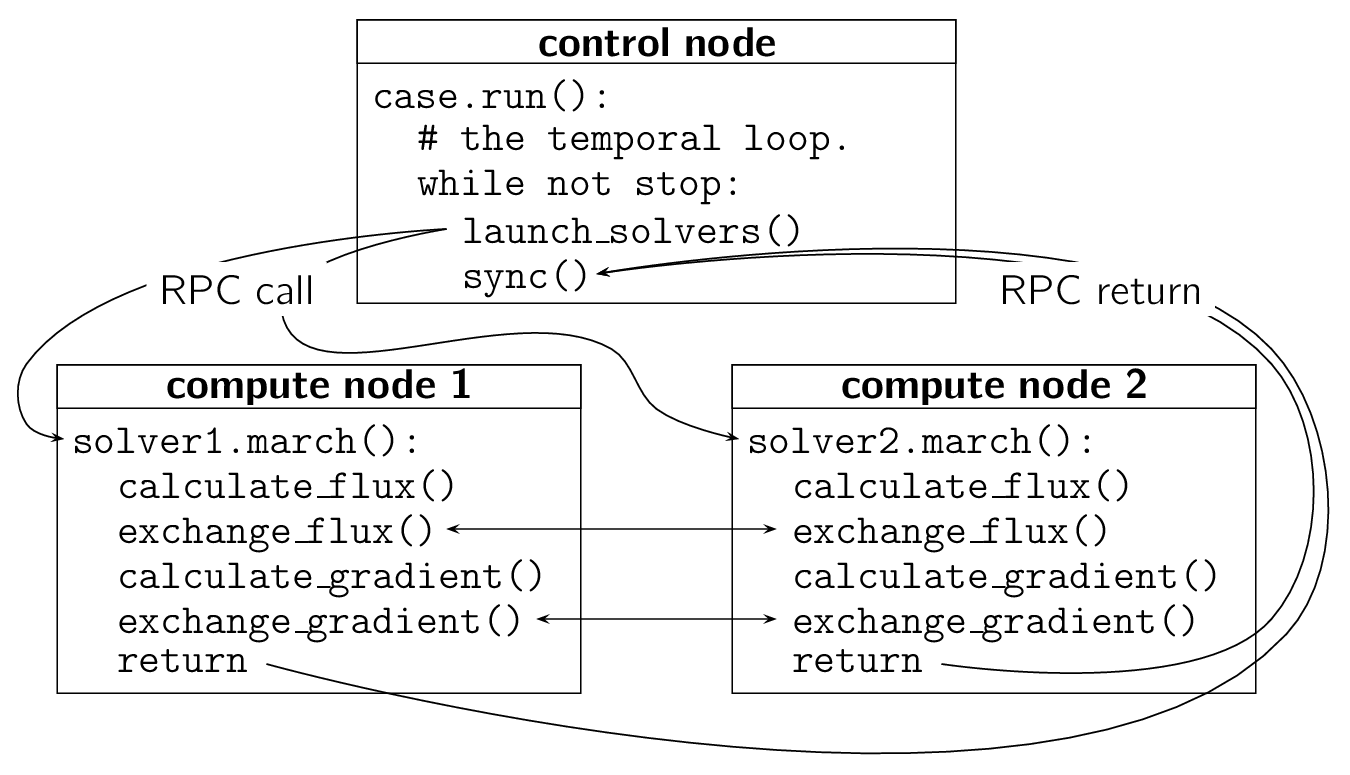
\includegraphics[width=\textwidth]{discomp.eps}
\end{column}
\end{columns}
\begin{itemize}
  \item When developing solver kernels, we do not need to worry about the
  complexity of DMPC.
  \item Hybrid parallelism is achieved by the segregation.
\end{itemize}
\end{frame}

\subsection{
%%
Treating ``Big Data''
%%
}

\begin{frame}{
%
Post-Processing is Bottleneck
%
}
\begin{itemize}
  \item High-resolution simulations generate a lot of data:
  \begin{itemize}
    \item For 50 million element mesh, the data for one scalar
    (single-precision) are \alert{200 MB}.
    \item A typical run has at least 10,000 time steps.
    \item Transient analysis: $10,000 \times 200 \,\mbox{MB} = \alert{2
    \,\mbox{TB}}$.
    \item $\rho, p, T, \vec{v}, \vec{\omega}$ for CFD: $2 \,\mbox{TB} \times 9 =
    \alert{18 \,\mbox{TB}}$.
  \end{itemize}
  \item Workaround: Reducing output frequency.
  \begin{itemize}
    \item Every 100 time steps: \alert{160 GB}.
  \end{itemize}
  \item Post-processing the solutions is painfully time-consuming:
  \begin{itemize}
    \item The large data are usually processed by using a single workstation.
    \item Turnaround time could be in months.
  \end{itemize}
\end{itemize}
\end{frame}

\begin{frame}{
%
Solutions in SOLVCON
%
}
\begin{itemize}
  \item Parallel I/O.
  \begin{itemize}
    \item Each sub-domain outputs its own solutions.
    \item It is used with \alert{parallel post-processing}.
  \end{itemize}
  \item In situ visualization.
  \begin{itemize}
    \item Visualization is being done on the fly with the simulation.
    \item Everything happens in memory.
    \item Output only graphic files, which are much smaller than the full
    solution field.
  \end{itemize}
  \item Parallel I/O and in situ visualization are complementary to each other.
\end{itemize}
\end{frame}

\section{
%%%
Example: Sod's Shock Tube
%%%
}

\begin{frame}{
%
Driving Scripts
%
}
\begin{itemize}
  \item Driving scripts manage simulations for SOLVCON.
  \begin{itemize}
    \item A driving script must create a \texttt{Case} object and call its (i)
    \texttt{init()}, (ii) \texttt{run()}, and (iii) \texttt{cleanup()} methods.
    \item No input file is needed.
  \end{itemize}
  \item Driving scripts can specify \alert{logic} to the simulations in addition to
  parameters.
  \begin{itemize}
    \item Anything higher than the foundation layer (the lowest layer) can be
    \alert{replaced} by code written in driving scripts.
    \item Including but not limited to \texttt{Case}, \texttt{Solver},
    \texttt{BC} classes, \texttt{Hook}, and \texttt{Anchor} classes.
  \end{itemize}
\end{itemize}
\end{frame}

\begin{frame}[fragile]{
%
Three-Dimensional Sod's Shock Tube
%
}
\begin{itemize}
  \item
  \href{https://bitbucket.org/solvcon/solvcon/src/09bcbc949751/examples/gasdyn/tube}{\texttt{\$SCROOT/examples/gasdyn/tube}}.
  \begin{itemize}
    \item The one-dimensional version is a standard test case for gas-dynamics
    codes.
    \item This version demonstrates the three-dimensional capability of
    SOLVCON.
    \item You also need \href{http://cubit.sandia.gov/}{CUBIT} to generate the
    mesh.
  \end{itemize}
  \item Let's go live demo.
\end{itemize}
\end{frame}

\begin{frame}[fragile]{
%
General Structure of a Driving Script
%
}
\begin{itemize}
  \item The driving script for the shock tube problem:
  \begin{Verbatim}[frame=single,numbers=left,fontsize=\scriptsize,commandchars=\\\{\}]
  from solvcon.kerpak import gasdyn
  class DiaphragmIAnchor(gasdyn.GasdynIAnchor):
      ...
  def tube_base(casename=None,
      gamma=None, rho1=None, p1=None, rho2=None, p2=None,
      psteps=None, ssteps=None, **kw
  ):
      ...
  if __name__ == '__main__':
      cse = tube_base('tube_20', use_incenter=True,
          gamma=1.4, rho1=1.0, p1=1.0, rho2=0.125, p2=0.25,
          time_increment=1.8e-3, steps_run=400, ssteps=40, psteps=1)
      cse.\alert{init()}
      cse.\alert{run()}
      cse.\alert{cleanup()}
  \end{Verbatim}
  \item There's another ``delayed'' mode for driving scripts.  See
  \href{https://bitbucket.org/solvcon/solvcon/src/09bcbc949751/examples/gasdyn/blnt}{examples/gasdyn/blnt}.
\end{itemize}
\end{frame}

\begin{frame}[fragile]{
%
Use Anchor for Initial Condition
%
}
\begin{itemize} \small
  \item The \texttt{provide()} method is invoked before the temporal loop:
  \begin{Verbatim}[frame=single,numbers=left,fontsize=\scriptsize,commandchars=\\\{\}]
  class DiaphragmIAnchor(gasdyn.GasdynIAnchor):
      ...
      def provide(self):
          super(DiaphragmIAnchor, self).provide()
          gamma = self.gamma
          svr = self.svr
          svr.soln[:,0].fill(self.rho1)
          svr.soln[:,1].fill(0.0)
          svr.soln[:,2].fill(0.0)
          if svr.ndim == 3:
              svr.soln[:,3].fill(0.0)
          svr.soln[:,svr.ndim+1].fill(self.p1/(gamma-1))
          # set.
          slct = svr.clcnd[:,0] > 0.0
          svr.soln[slct,0] = self.rho2
          svr.soln[slct,svr.ndim+1] = self.p2
          # update.
          svr.sol[:] = svr.soln[:]
  \end{Verbatim}
\end{itemize}
\end{frame}

\begin{frame}[fragile]{
%
Setup the Simulation
%
}
\begin{itemize} \small
  \item A \texttt{Case} object is created for the simulation:
  \begin{Verbatim}[frame=single,numbers=left,fontsize=\scriptsize]
  def tube_base(...):
      ...
      # set up case.
      basedir = os.path.abspath(os.path.join(os.getcwd(), 'result'))
      cse = gasdyn.GasdynCase(basedir=basedir, rootdir=env.projdir,
          basefn=casename, mesher=mesher, bcmap=bcmap, **kw)
      # informative.
      cse.runhooks.append(hook.BlockInfoHook)
      ...
      # initializer.
      ...
      cse.runhooks.append(DiaphragmIAnchor,
          gamma=gamma, rho1=rho1, p1=p1, rho2=rho2, p2=p2)
      # post processing.
      ...
      cse.runhooks.append(gasdyn.GasdynOAnchor, rsteps=ssteps)
      ...
      return cse
  \end{Verbatim}
\end{itemize}
\end{frame}

\section{
%%%
Conclusions
%%%
}

\begin{frame}{
%
A Planned Renovation of SOLVCON
%
}
\begin{center}
  \parbox{\textwidth}{\centering
  \includegraphics[width=0.9\textwidth]{stack_planned.eps}}
\end{center}
\begin{itemize} \footnotesize
  \item Simply the architecture: Rely more on mpi4py, OpenMP, etc.
  \item Use Cython instead of ctypes for maintainability.
\end{itemize}
\end{frame}

\begin{frame}{
%
Conclusions
%
}
\begin{itemize}
  \item For computational scientists, Python is the way to go.
  \begin{itemize}
    \item I've done all the presented results by myself.
    \item It's very \alert{productive}.
  \end{itemize}
  \item Download the source files of the slides: \url{http://j.mp/P06kl9}
\end{itemize}
\end{frame}

\end{document}

% vim: set spell:
